\documentclass[border=3pt]{standalone}
\usepackage{siunitx}
\usepackage[compat=1.1.0]{tikz-feynman}
\usepackage{amsmath, mathtools}
\begin{document}
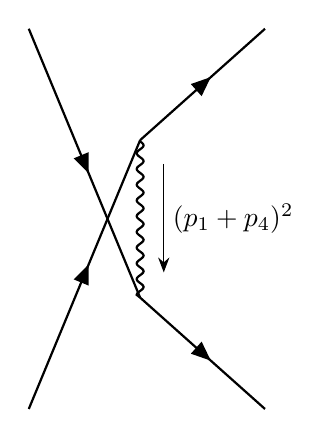
\begin{tikzpicture}
  \begin{feynman}[large]
    \vertex (a);
    \vertex [below      =of a] (b);
    \vertex [above left=of a] (i1);
    \vertex [below left =of b] (i2);
    \vertex [right      =3cm of i2] (f1);
    \vertex [right      =3cm of i1] (f2);

    \diagram* {
      (i1) -- [fermion] (b)
           -- [fermion] (f1),
      (a) -- [photon, momentum={\((p_1+p_4)^2\)}] (b),
      (i2) -- [fermion] (a),
      (a) -- [fermion] (f2),
    };
  \end{feynman}
\end{tikzpicture}
\end{document}
